
\documentclass{article}

\usepackage[pdftex]{graphicx}
%\usepackage{graphicx}
%\usepackage{amsmath}
\usepackage{url}
%\usepackage{apacite}
%\usepackage{mslapa}

\begin{document}

\title{Experiments in Tuning an Automotive Engine}
\author{Jeremiah Mahler}
\date{\today}

\maketitle

\tableofcontents

\pagebreak

\section{Preface}

The spectrum of settings in which an engine will run is large
but there is only one set of settings that is optimal.

This document describes the techniques that were developed
for optimizing the settings of an engine.
This was in conjuction with the development of the
Msqdev \cite{MAHL11} system which provides an interface for
automated tuning of a Megasquirt \cite{MEGA11} based ecu.
\nocite{R}

\section{Constant Idle Speed Tuning, Maximize Rpm}
% June 10, 2011

When an engine is at idle (with no adaptive idle control) at a constant
throttle position and constant load, any change in fuel or ignition
should have a direct change in engine rpm.
And a higher rpm would indicate that more power being produced.

\begin{figure}[!hbt]
\center
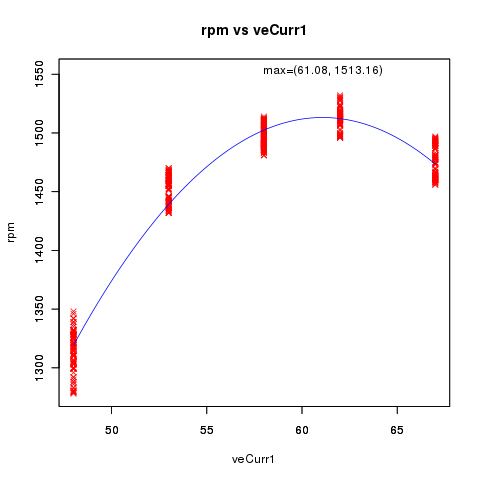
\includegraphics[scale=0.5]{plot01}
\caption{Varying veCurr1 vs rpm at idle.}
\end{figure}

\section{Constant Road Speed Tuning, Excessive Error}
\label{roaderr}

It should be possible to drive a car at a steady speed (constant throttle
position) while allowing the settings to be varied.
And the results should provide peaks at various points through out the map.

Testing was performed by driving a car on a flat road at a steady speed
and then allowing points to be varied.

Several problems appeared during testing.
The first is that it is very difficult for a person to precisely
position the throttle.
Any slight movement will cause a disruption of the position.
The second is in detecting slight amounts of acceleration.
Because the amount of change from varying settings is on the order 
of 100 rpm even the slightests acceleration will ruin the results.

These problems did reveal a benefit of the current setting variation
algorithm.
Previously settings were varied from a left extreme to a right extreme.
Currently settings are varied from the center to the left extreme,
then back to the center and to the right extreme.
The benefit of the current algorithm is that the center point will
indicate if any errors occured.
If no error occured the center point will be the same during both times
it is tested.
If an error occurs, such as acceleration, the center points will be
shifted apart (see Figure \ref{fig:ssrerr}).

\begin{figure}[!htb]
\center
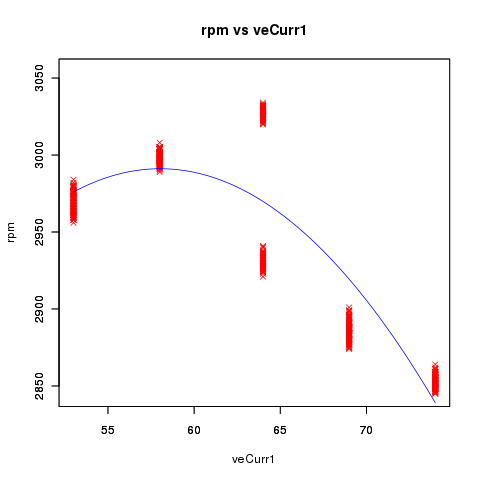
\includegraphics[scale=0.5]{plotdata-veTable1-20110613-15:17:10.png}
\caption{Constant road speed tuning with a large error (deceleration)
indicated by the center left right algorithm.}
\label{fig:ssrerr}
\end{figure}

\section{Constant Road Speed Tuning with a Throttle Stop}
\label{sec:tstop}
% June 15, 2011

To minimize the error caused by a human driver controlling the throttle
(as was discussed in Section \ref{roaderr})
rigid stops are used underneath the gas pedal to provide a fixed
depressed position.
The stops were cut from tubing in to various lengths and they
can be substituted as approperiate for a given test.
It should be possible to substitute different length stops and
the engine rpm should stabilize at different points.

Testing on level ground revealed that only one of the stops, which
corresponded to a very slight throttle opening, would result in
a stable engine rpm.
All the other stops resulted in steady acceleration of varying degrees.
The throttle stops of larger openings would need an increased load,
such as from an incline, in order for the engine rpm to stabilize.

The tuning results show a significant increase in precision.
There was no discernable separation in the center point
indicating there is a very low amount of error (see Figure \ref{fig:tstop}).

\begin{figure}[!htb]
\center
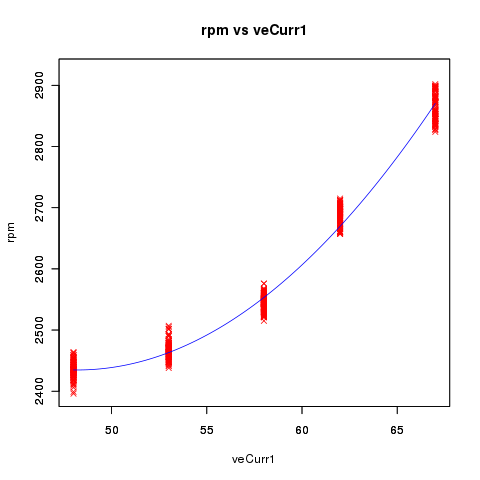
\includegraphics[scale=0.5]{20110615-throttle_stop.png}
\caption{Variation of settings while using a throttle stop.}
\label{fig:tstop}
\end{figure}

The throttle stop is clearly a valuable addition to steady
state tuning and should be used in all testing situations.

\section{Constant Road Speed Tuning Impractical}
% June 16, 2011
%After many attempts to tune at a constant road speed it has
%been determined it is impractical.

For a given load there is a single throttle position in which
the rpm will stabilize and the speed will remain constant.
Because the throttle stops (Section \ref{sec:tstop}) are a fixed
imprecise size and are not easy to adjust it is too difficult
to maintain a constant speed.

Constant acceleration tuning (Section \ref{sec:conacc})
should be more forgiving in this respect because it does not require
stabilization and it is not depenent on any specific throttle position
or load.

\section{Constant Acceleration}
\label{sec:conacc}
(in development)

Under a constant load and a constant throttle position
(assuming the throttle position is such to cause acceleration)
a constant acceleration should result.
Strictly speaking the acceleration will not be constant due to
changes in load and varying performance of the engine.
For the purposes of this document this term will be used to
refer to acceleration as opposed to no acceleration.

In contrast to steady state tuning where a single setting is varied
at a single point, acceleration goes through through many points
and there is not enough time to vary the settings at each point.
If two trials are performed under the same conditions (load and throttle
position) with different settings these trials can be compared.

One difficulty with this method is having to align the data for comparison.
Perhaps a starting and ending rpm range with a constant throttle position
throughout.

If optimizing for maximum power using a plot of rpm versus time the settings
with the highest rpm in the shortest period of time would be the optimal
solution.  An integral could be used to find the area and the settings with
the largest area would have the greates acceleration.

Unlike steady state tuning this method does not lend it self to hill climbing.
Since many variables are changed it may be better solved using Genetic Algorithms.

\section{throttle response}
(in development)

The biggest difficulty with tuning throttle response is producing
a repeatable movement of the throttle.
One possible solution is to record all the different types and then
when a match is found with different settings it can be used for
comparison.
Another possibility is to build a mechanical apparatus using a solenoid
or some other device which precisely actuates the throttle.

\pagebreak

%\bibliographystyle{mslapa}
%\bibliographystyle{plain}
%\bibliographystyle{acm}
\bibliographystyle{ieeetr}
\bibliography{main}

\end{document}
